\section{Experiments}
\label{sec:experiments}

We evaluate CyCADA on several unsupervised adaptation scenarios. We first focus on adaptation for digit classification using the MNIST~\citep{lecun_ieee98}, USPS, and Street View House Numbers (SVHN)~\citep{netzer_nips11} datasets. After which we present results for the task of semantic image segmentation, using the SYNTHIA~\citep{ros_cvpr16}, GTA~\citep{richter_eccv16} and CityScapes~\citep{cordts_cvpr16} datasets. 

\subsection{Digit Adaptation}
We evaluate our method across the adaptation shifts of USPS to MNIST, MNIST to USPS, and SVHN to MNIST, using the full training sets during learning phases and evaluating on the standard test sets. We report classification accuracy for each shift in Table~\ref{table:digits} and find that our method outperforms competing approaches on average. 
The classifier for our method for all digit shifts uses a variant of the LeNet architecture (see \ref{sec:digit-details} for full implementation details). 
Note that the recent pixel-da method by \citet{bousmalis_cvpr17} presents results for only the MNIST to USPS shift and reports 95.9\% accuracy, while our method achieves 95.6\% accuracy. However, the pixel-da approach cross validates with some labeled data which is not an equivalent evaluation setting. 

\textbf{Ablation: Pixel vs Feature Level Transfer.} We begin by evaluating the contribution of the pixel space and feature space transfer. 
We find that in the case of the small domain shifts between USPS and MNIST, the pixel space adaptation by which we train a classifier using images translated using CycleGAN~\citep{zhu_arxiv17}, performs very well, outperforming or comparable to prior adaptation approaches. 
Feature level adaptation offers a small benefit in this case of a small pixel shift. 
However, for the more difficult shift of SVHN to MNIST, we find that feature level adaptation outperforms the pixel level adaptation, and importantly, both may be combined to produce an overall model which outperforms all competing methods. 

\begin{table}
  \centering
  \scriptsize
  \setlength{\tabcolsep}{1.35pt}
  \begin{tabular}{lccc}
    \toprule
	Model & 		MNIST $\rightarrow$ USPS & USPS $\rightarrow$ MNIST & SVHN $\rightarrow$ MNIST \\
	\midrule \midrule
	Source only & 	82.2 $\pm$ 0.8 &  69.6 $\pm$ 3.8 &	67.1 $\pm$ 0.6\\
	DANN~\citep{dann}&	-	&	-	&73.6\\
	DTN~\citep{dtn} &	-&		-&	84.4\\
	CoGAN~\citep{cogan} &	91.2 &	89.1 &	-\\
	ADDA~\citep{tzeng_cvpr17} & 	89.4 $\pm$ 0.2 &	90.1 $\pm$ 0.8 &	76.0 $\pm$ 1.8\\
	
        %PixelDA~\citep{bousmalis_cvpr17} & \bf 95.9 & - & -  \\
        CyCADA pixel only & 	 \bf 95.6 $\pm$ 0.2 &	96.4 $\pm$ 0.1&	70.3 $\pm$ 0.2\\
	%CyCADA pixel only w/ $\mathcal{L}_{\text{sem}}$ & 	-	&	-	&	71.15 $\pm$ 0.4\\
	CyCADA pixel+feat & 	\bf  95.6 $\pm$ 0.2 & 	\bf	96.5 $\pm$ 0.1 &	\bf	90.4 $\pm$ 0.4\\
	\midrule
	Target only & 	96.3 $\pm$ 0.1 & 	99.2 $\pm$ 0.1&	99.2 $\pm 0.1$\\
    \bottomrule
  \end{tabular}
  \caption{
    %\small
    \textbf{Unsupervised domain adaptation across digit datasets.} Our model is competitive with or outperforms state-of-the-art models for each shift. For the difficult shift of SVHN to MNIST we also note that feature space adaptation provides additional benefit beyond the pixel-only adaptation. 
    }
  \label{table:digits}
\end{table}

\begin{figure}
	\centering
	\begin{tabular}{cc}
	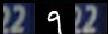
\includegraphics[height=.1\linewidth]{figs/svhn2mnist_cyclegan_bad_cycle3.jpeg} &
	
\includegraphics[height=.1\linewidth]{figs/digit-ablation/no-cycle/1_00000_real_B.png}
	
\includegraphics[height=.1\linewidth]{figs/digit-ablation/no-cycle/1_00000_fake_A.png}
	
\includegraphics[height=.1\linewidth]{figs/digit-ablation/no-cycle/1_00000_rec_B.png}
	\\
	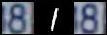
\includegraphics[height=.1\linewidth]{figs/svhn2mnist_cyclegan_bad_cycle4.jpeg} &
	
\includegraphics[height=.1\linewidth]{figs/digit-ablation/no-cycle/4_00026_real_B.png}
	
\includegraphics[height=.1\linewidth]{figs/digit-ablation/no-cycle/4_00026_fake_A.png}
	
\includegraphics[height=.1\linewidth]{figs/digit-ablation/no-cycle/4_00026_rec_B.png}\\
	(a) Without Semantic Loss & (b) Without Cycle Loss
	\end{tabular}
	\caption{\textbf{Ablation: Effect of Semantic or Cycle Consistency} Examples of translation failures without the semantic consistency loss. Each triple contains the original SVHN image (\textit{left}), the image translated into MNIST style (\textit{middle}), and the image reconstructed back into SVHN (\textit{right}). (a) Without semantic loss, both the GAN and cycle constraints are satisfied (translated image matches MNIST style and reconstructed image matches original), but the image translated to the target domain lacks the proper semantics. (b) Without cycle loss, the reconstruction is not satisfied and though the semantic consistency leads to some successful semantic translations (\textit{top}) there are still cases of label flipping (\textit{bottom}).}
	\label{fig:cyclegan_fail}
\end{figure}

\textbf{Ablation: No Semantic Consistency.} We experiment without the addition of our semantic consistency loss and find that the standard unsupervised CycleGAN approach diverged when training SVHN to MNIST often suffering from random label flipping.
 Figure~\ref{fig:cyclegan_fail}(a) demonstrates two examples where cycle constraints alone fail to have the desired behavior for our end task. An SVHN image is mapped to a convincing MNIST type image and back to a SVHN image with correct semantics. However, the MNIST-like image has mismatched semantics. Our modified version, which uses the source labels to train a weak classification model which can be used to enforce semantic consistency before and after translation, resolves this issue and produces strong performance.
 
 \textbf{Ablation: No Cycle Consistency.} We study the result when learning without the cycle consistency loss. First note that there is no reconstruction guarantee in this case, thus in Figure~\ref{fig:cyclegan_fail}(b) we see that the translation back to SVHN fails. In addition, we find that while the semantic loss does encourage correct semantics it relies on the weak source labeler and thus label flipping still occurs (see right image triple).



\subsection{Semantic Segmentation Adaptation}
The task is to assign a semantic label to each pixel in the input image, e.g. $road$, $building$, etc.
We limit our evaluation to the unsupervised adaptation setting, where labels are only available in the source domain, but we are evaluated solely on our performance in the target domain.

For each experiment, we use three metrics to evaluate performance.
Let $n_{ij}$ be the number of pixels of class $i$ predicted as class $j$, let $t_i = \sum_j n_{ij}$ be the total number of pixels of class $i$, and let $N$ be the number of classes.
Our three evaluation metrics are, mean intersection-over-union (mIoU), frequency weighted intersection-over-union (fwIoU), and pixel accuracy, which are defined as follows: \\
mIoU $=\frac{1}{N} \cdot \frac{\sum_i n_{ii}}{t_i + \sum_j n_{ji} - n_{ii}}$, fwIoU $=\frac{1}{\sum_k t_k} \cdot \frac{\sum_i n_{ii}}{t_i + \sum_j n_{ji} - n_{ii}}$, pixel acc. $=\frac{\sum_i n_{ii}}{\sum_i t_i}$.

Cycle-consistent adversarial adaptation is general and can be applied at any layer of a network. 
Since optimizing the full CyCADA objective in Equation~\ref{eq:cycada} end-to-end is memory-intensive in practice, we train our model in stages.
First, we perform image-space adaptation and map our source data into the target domain.
Next, using the adapted source data with the original source labels, we learn a task model that is suited to operating on target data.
Finally, we perform another round of adaptation between the adapted source data and the target data in feature-space, using one of the intermediate layers of the task model. Additionally, we do not use the semantic loss for the segmentation experiments as it would require loading generators, discriminators, and an additional semantic segmenter into memory all at once for two images. We did not have the required memory for this at the time of submission, but leave it to future work to deploy model parallelism or experiment with larger GPU memory. 


For our first evaluation, 
we consider the SYNTHIA dataset~\citep{ros_cvpr16}, which contains synthetic renderings of urban scenes.
We use the SYNTHIA video sequences, which are rendered across a variety of environments, weather conditions, and lighting conditions.
This provides a synthetic testbed for evaluating adaptation techniques.
For comparison with previous work, in this work we focus on adaptation between seasons.
We use only the front-facing views in the sequences so as to mimic dashcam imagery, and adapt from fall to winter.
The subset of the dataset we use contains 13 classes and consists of 10,852 fall images and 7,654 winter images.

To further demonstrate our method's applicability to real-world adaptation scenarios, we also evaluate our model in a challenging synthetic-to-real adaptation setting.
For our synthetic source domain, we use the GTA5 dataset~\citep{richter_eccv16} extracted from the game Grand Theft Auto V, which contains 24966 images. 
We consider adaptation from GTA5 to the real-world Cityscapes dataset~\citep{cordts_cvpr16}, from which we used 19998 images without annotation for training and 500 images for validation. 
Both of these datasets are evaluated on the same set of 19 classes, allowing for straightforward adaptation between the two domains.

Image-space adaptation also affords us the ability to visually inspect the results of the adaptation method.
This is a distinct advantage over opaque feature-space adaptation methods, especially in truly unsupervised settings---without labels, there is no way to empirically evaluate the adapted model, and thus no way to verify that adaptation is improving task performance.
Visually confirming that the conversions between source and target images are reasonable, while not a \emph{guarantee} of improved task performance, can serve as a sanity check to ensure that adaptation is not completely diverging. This process is diagrammed in Figure~\ref{fig:implementation}. For implementation details please see Appendix \ref{sec:ss-details}.





\newcommand{\myw}{3.5cm}
\newcommand{\myh}{1.8cm}
\subsubsection{Cross-season adaptation}

We start by exploring the abilities of pixel space adaptation alone (using FCN8s architecture) for the setting of adapting across seasons in synthetic data. For this we use the SYNTHIA dataset and adapt from fall to winter weather conditions. 
Typically in unsupervised adaptation settings it is difficult to interpret what causes the performance improvement after adaptation.
Therefore, we use this setting as an example where we may directly visualize the shift from fall to winter and inspect the intermediate pixel level adaptation result from our algorithm.
In Figure~\ref{fig:synthia} we show the result of pixel only adaptation as we generate a winter domain image (b) from a fall domain image (a), and visa versa (c-d). We may clearly see the changes of adding or removing snow. This visually interpretable result matches our expectation of the true shift between these domains and indeed results in favorable final semantic segmentation performance from fall to winter as shown in Table~\ref{table:synthia}. We find that CyCADA achieves state-of-the-art performance on this task with image space adaptation alone, however does not recover full supervised learning performance (train on target). Some example errors includes adding snow to the sidewalks, but not to the road, while in the true winter domain snow appears in both locations. However, even this mistake is interesting as it implies that the model is learning to distinguish road from sidewalk during pixel adaptation, despite the lack of pixel annotations.

\begin{table*}
  \centering
  \scriptsize
  \setlength{\tabcolsep}{3.0pt}
  \begin{tabular}{l|cccccccccccccggg}
    \toprule
    \multicolumn{17}{c}{\textbf{SYNTHIA Fall $\rightarrow$ Winter}} \\
    \midrule
    & \rot{sky} & \rot{building} & \rot{road} & \rot{sidewalk} & \rot{fence} & \rot{vegetation} & \rot{pole} & \rot{car} & \rot{traffic sign} & \rot{pedestrian} & \rot{bicycle} & \rot{lanemarking} & \rot{traffic light} & \rot{\textbf{mIoU}} & \rot{\textbf{fwIoU}} & \rot{\textbf{Pixel acc.}} \\ \midrule
    %\# of instances & 19 & 96 & 87 & 210 & 611 & 103 & 122 & 129 & 25 & 55 & 144 & 37 & 51 & 276 & 47 & 129 & 210 & 33 & 17 & 2401 \\ \midrule
    Source only            & 91.7 & 80.6 & 79.7 & 12.1 & 71.8 & 44.2 & 26.1 & 42.8 & 49.0 & 38.7 & 45.1 & 41.3 & 24.5 & 49.8 & 71.7 & 82.3 \\
    % \cite{hoffman_arxiv16} & 94.5 & 87.0 & 84.0 & 46.5 & 62.7 & 65.8 & 51.0 & 68.1 & 55.7 & 58.5 & 53.9 & 48.3 & 30.8 & 62.0 \\ I goofed and this is W -> F
    FCNs in the wild & 92.1 & 86.7 & 91.3 & 20.8 & 72.7 & \textbf{52.9} & \textbf{46.5} & 64.3 & \textbf{50.0} & \textbf{59.5} & \textbf{54.6} & \textbf{57.5} & \textbf{26.1} & 59.6 &  --- &  --- \\
    CyCADA pixel-only    & \textbf{92.5} & \textbf{90.1} & \textbf{91.9} & \textbf{79.9} & \textbf{85.7} & 47.1 & 36.9 & \textbf{82.6} & 45.0 & 49.1 & 46.2 & 54.6 & 21.5 & \textbf{63.3} & \textbf{85.7} & \textbf{92.1} \\ \midrule
    Oracle (Train on target)        & 93.8 & 92.2 & 94.7 & 90.7 & 90.2 & 64.4 & 38.1 & 88.5 & 55.4 & 51.0 & 52.0 & 68.9 & 37.3 & 70.5 & 89.9 & 94.5 \\
    \bottomrule
  \end{tabular}
  \caption{
    Adaptation between seasons in the SYNTHIA dataset. We report IoU for each class and mean IoU, freq-weighted IoU and pixel accuracy.
    Our CyCADA method achieves state-of-the-art performance on average across all categories.  $^*$FCNs in the wild is by \citet{hoffman_arxiv16}.
    %\et[inline]{Bold numbers}
    }
  \label{table:synthia}
\end{table*}

\begin{table*}
  \centering
  \scriptsize
  \setlength{\tabcolsep}{3.0pt}
  \begin{tabular}{l|cccccccccccccggg}
    \toprule
    \multicolumn{17}{c}{\textbf{SYNTHIA Fall $\rightarrow$ Winter}} \\
    \midrule
    & \rot{sky} & \rot{building} & \rot{road} & \rot{sidewalk} & \rot{fence} & \rot{vegetation} & \rot{pole} & \rot{car} & \rot{traffic sign} & \rot{pedestrian} & \rot{bicycle} & \rot{lanemarking} & \rot{traffic light} & \rot{\textbf{mIoU}} & \rot{\textbf{fwIoU}} & \rot{\textbf{Pixel acc.}} \\ \midrule
    %\# of instances & 19 & 96 & 87 & 210 & 611 & 103 & 122 & 129 & 25 & 55 & 144 & 37 & 51 & 276 & 47 & 129 & 210 & 33 & 17 & 2401 \\ \midrule
    Source only            & 91.7 & 80.6 & 79.7 & 12.1 & 71.8 & 44.2 & 26.1 & 42.8 & 49.0 & 38.7 & 45.1 & 41.3 & 24.5 & 49.8 & 71.7 & 82.3 \\
    % \cite{hoffman_arxiv16} & 94.5 & 87.0 & 84.0 & 46.5 & 62.7 & 65.8 & 51.0 & 68.1 & 55.7 & 58.5 & 53.9 & 48.3 & 30.8 & 62.0 \\ I goofed and this is W -> F
    FCNs in the wild & 92.1 & 86.7 & 91.3 & 20.8 & 72.7 & \textbf{52.9} & \textbf{46.5} & 64.3 & \textbf{50.0} & \textbf{59.5} & \textbf{54.6} & \textbf{57.5} & \textbf{26.1} & 59.6 &  --- &  --- \\
    CyCADA pixel-only    & \textbf{92.5} & \textbf{90.1} & \textbf{91.9} & \textbf{79.9} & \textbf{85.7} & 47.1 & 36.9 & \textbf{82.6} & 45.0 & 49.1 & 46.2 & 54.6 & 21.5 & \textbf{63.3} & \textbf{85.7} & \textbf{92.1} \\ \midrule
    Oracle (Train on target)        & 93.8 & 92.2 & 94.7 & 90.7 & 90.2 & 64.4 & 38.1 & 88.5 & 55.4 & 51.0 & 52.0 & 68.9 & 37.3 & 70.5 & 89.9 & 94.5 \\
    \bottomrule
  \end{tabular}
  \caption{
    Adaptation between seasons in the SYNTHIA dataset. We report IoU for each class and mean IoU, freq-weighted IoU and pixel accuracy.
    Our CyCADA method achieves state-of-the-art performance on average across all categories.  $^*$FCNs in the wild is by \citet{hoffman_arxiv16}.
    %\et[inline]{Bold numbers}
    }
  \label{table:synthia}
\end{table*}

Cycle-consistent adversarial adaptation achieves state-of-the-art adaptation performance.
We see that under the fwIoU and pixel accuracy metrics, CyCADA approaches oracle performance, falling short by only a few points, despite being entirely unsupervised.
This indicates that CyCADA is extremely effective at correcting the most common classes in the dataset.
This conclusion is supported by inspection of the individual classes in Table~\ref{table:synthia}, where we see the largest improvement on common classes such as \emph{road} and \emph{sidewalk}.

\begin{figure}
  \centerline{
    \setlength{\tabcolsep}{2.0pt}
  \begin{tabular}{cccc}
    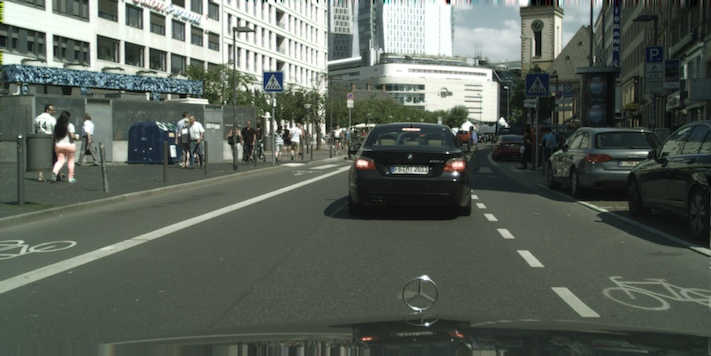
\includegraphics[width=\myw, height=\myh]{figs/gta2city_color/4_img.png} &
	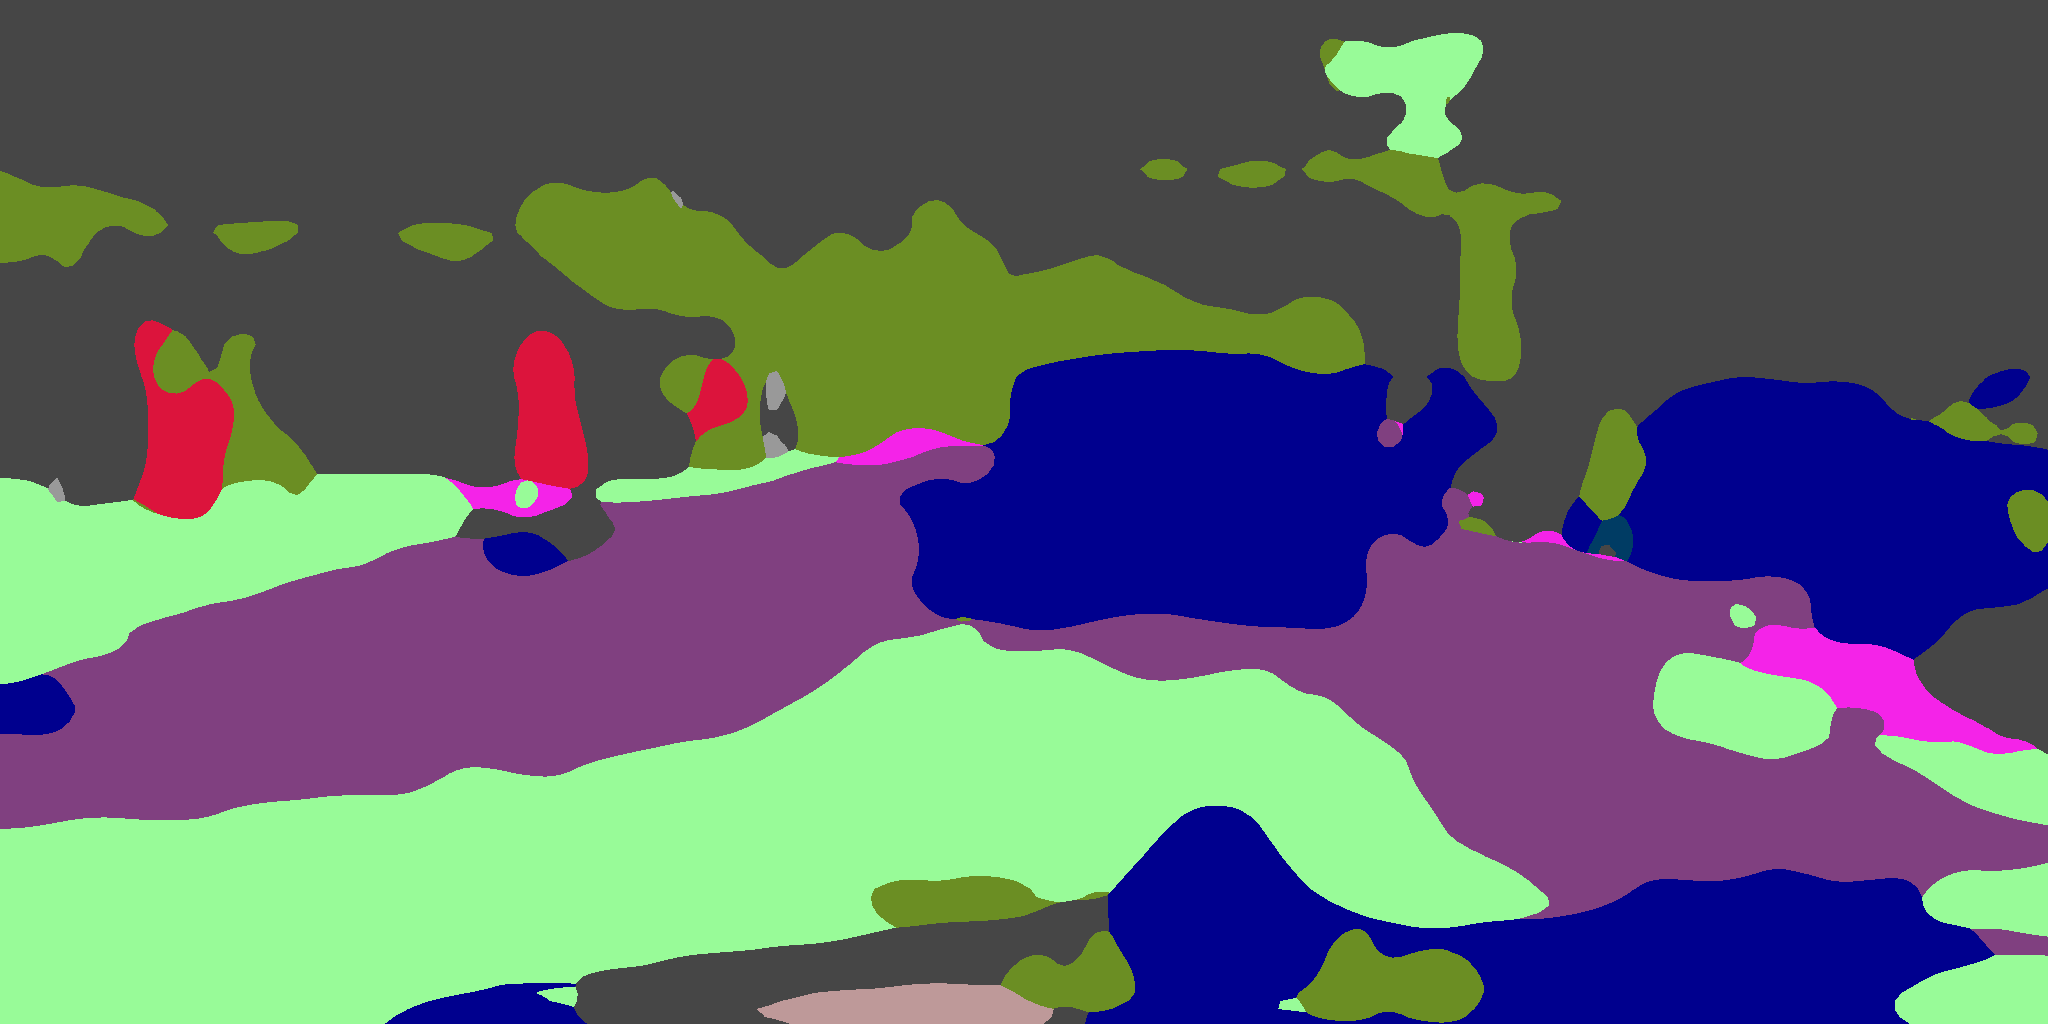
\includegraphics[width=\myw, height=\myh]{figs/gta2city_color/4_src.png} &
	
\includegraphics[width=\myw, height=\myh]{figs/gta2city_color/4_cycada.png} &
	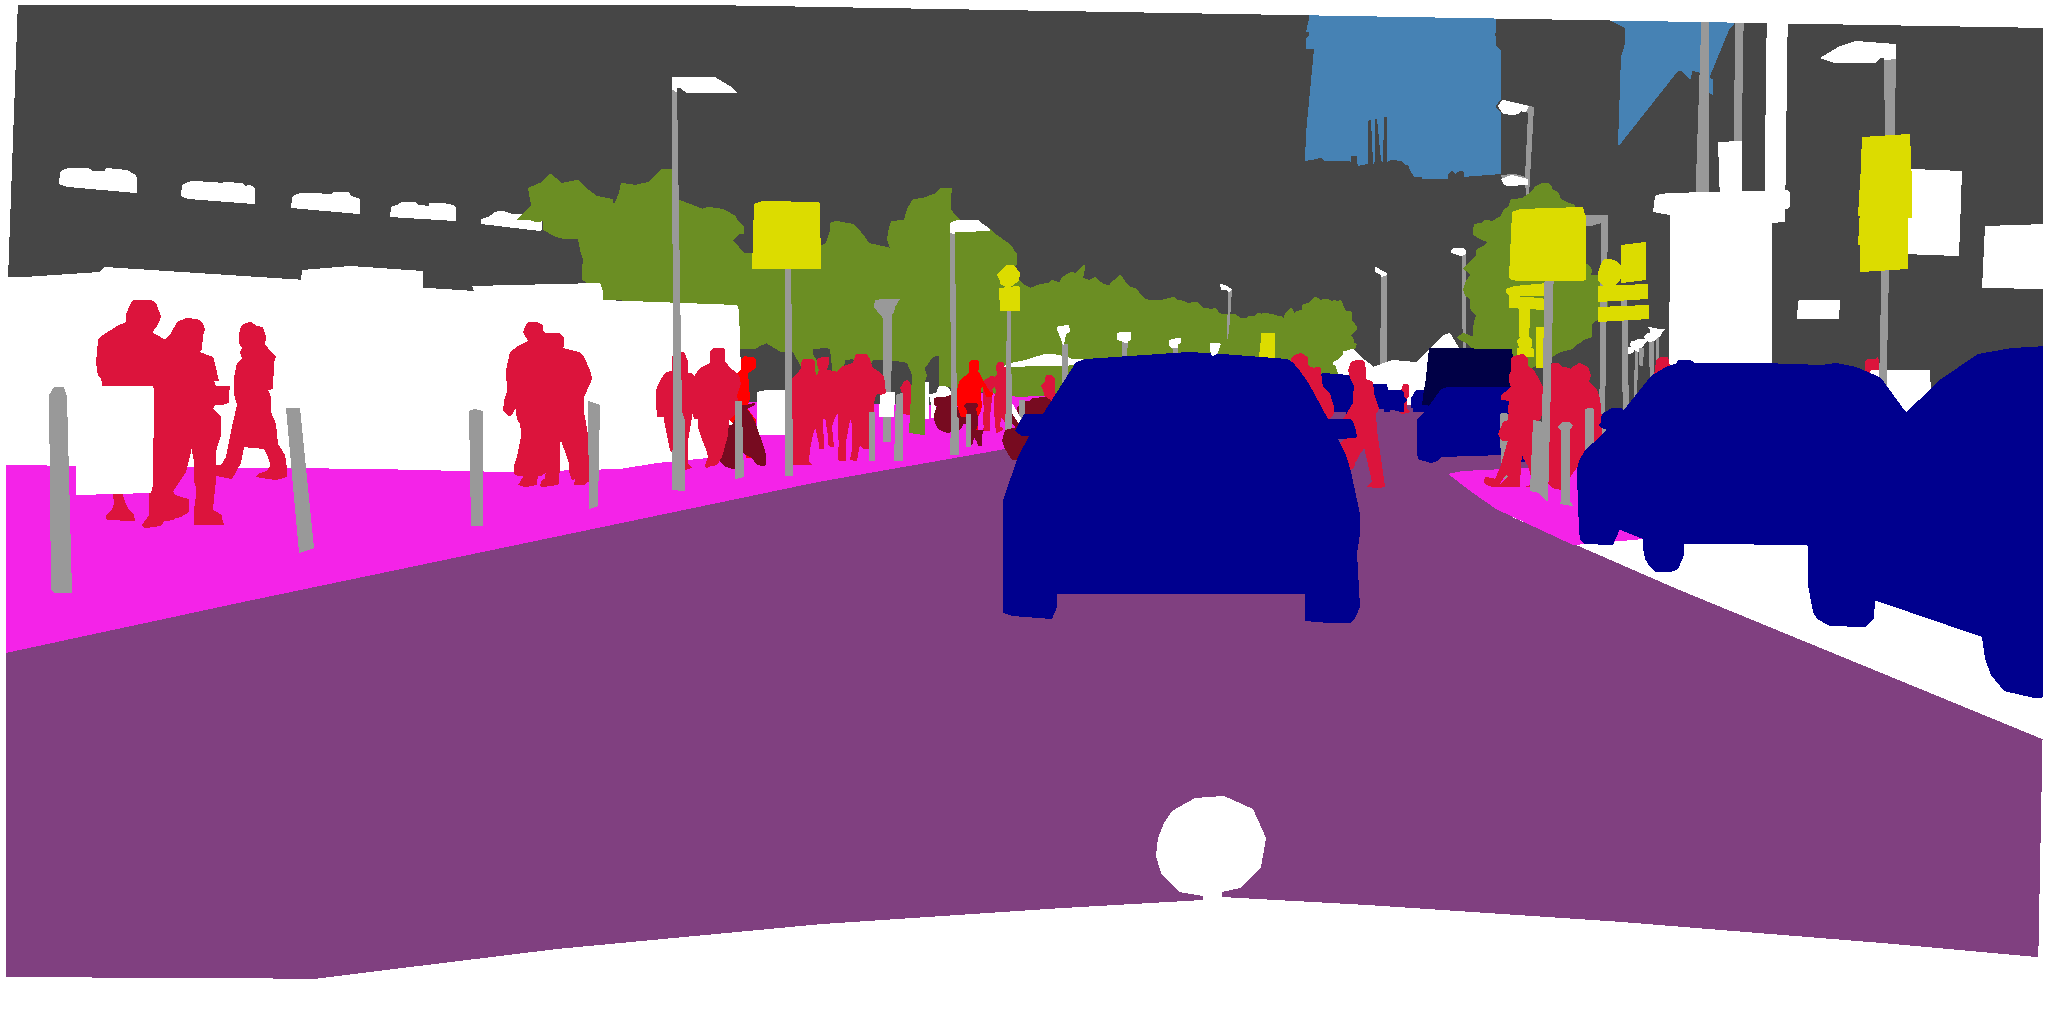
\includegraphics[width=\myw, height=\myh]{figs/gta2city_color/4_gt.png} 
   \\
   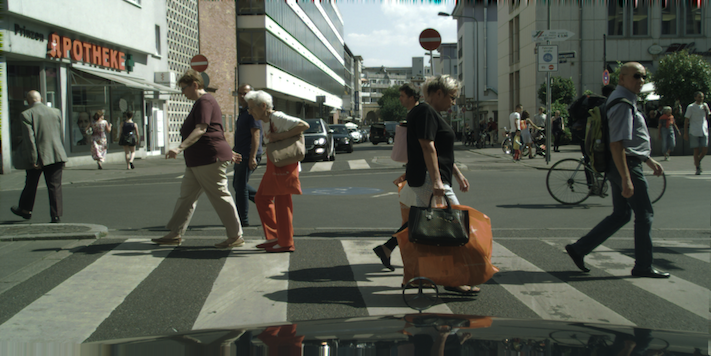
\includegraphics[width=\myw, height=\myh]{figs/gta2city_color/25_img.png} &

\includegraphics[width=\myw, height=\myh]{figs/gta2city_color/25_src.png} &
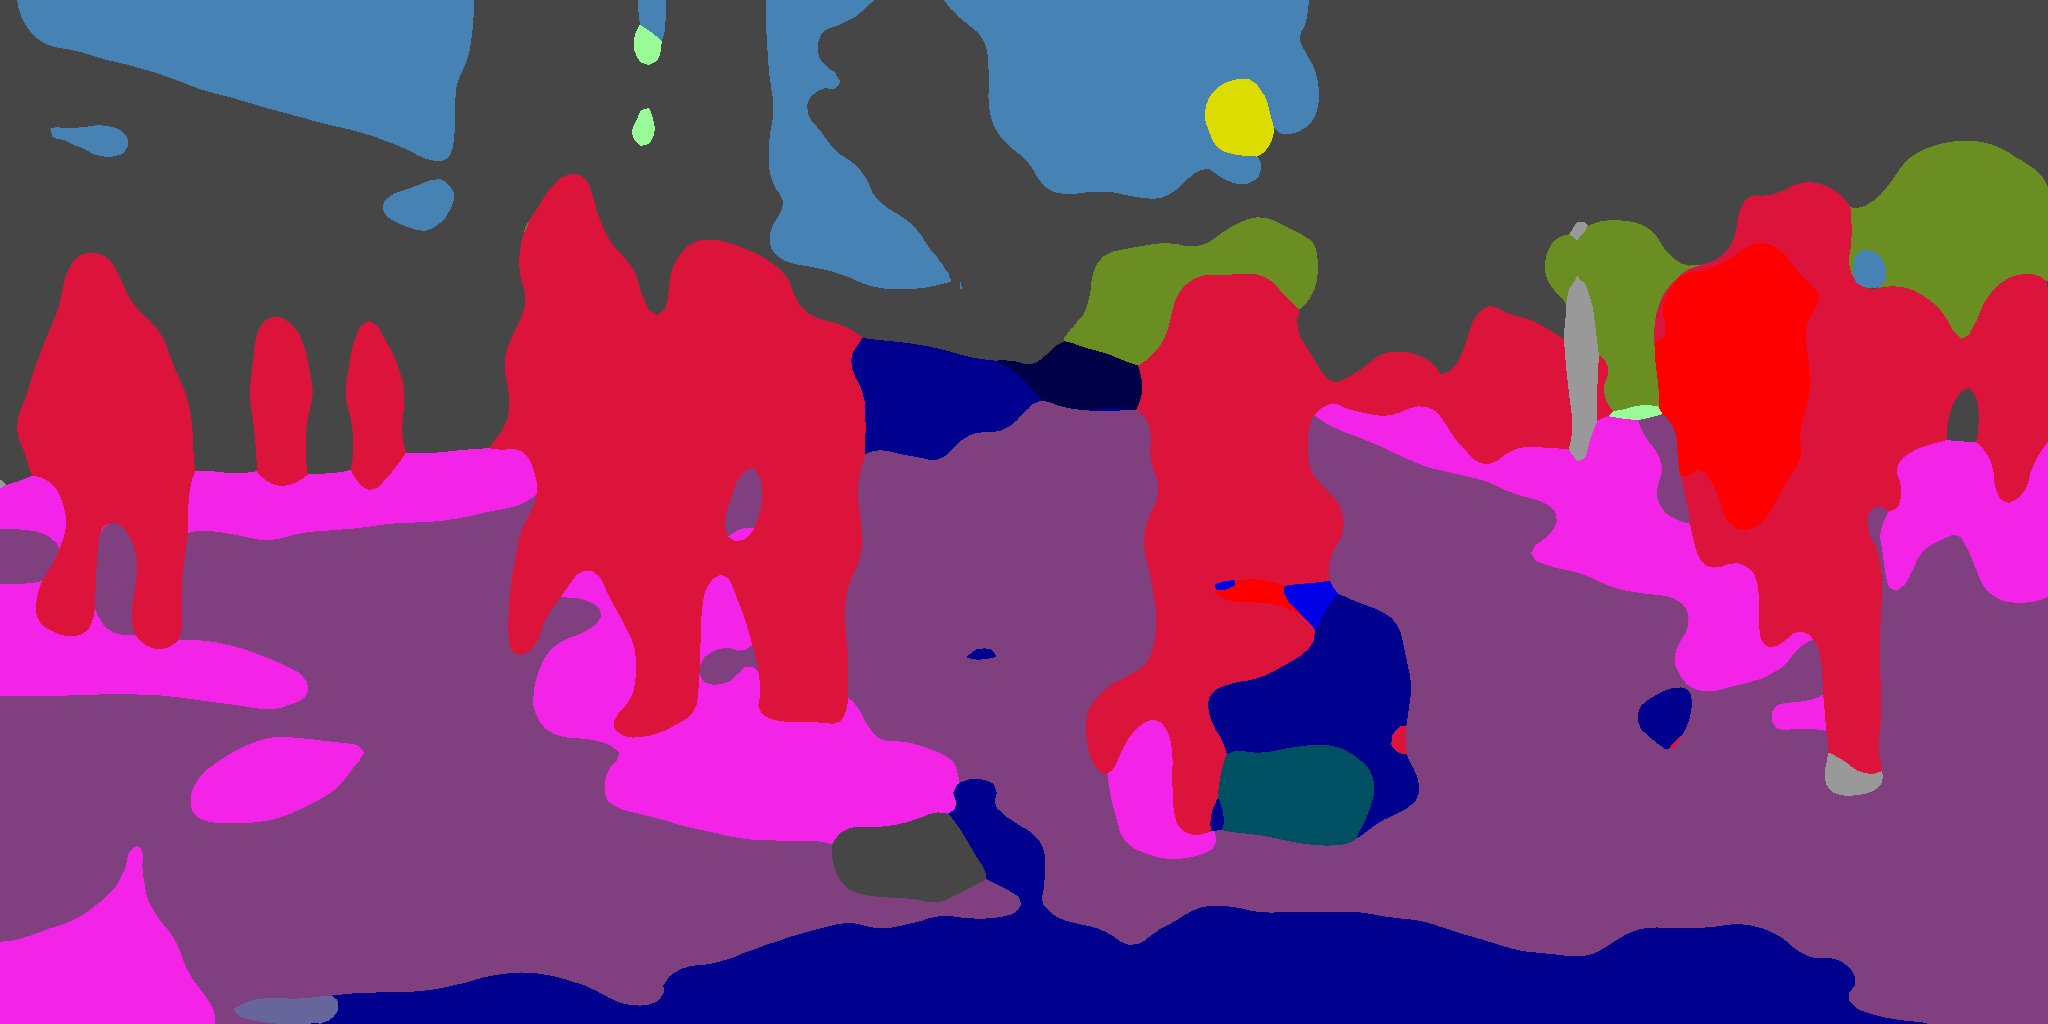
\includegraphics[width=\myw, height=\myh]{figs/gta2city_color/25_cycada.png} &
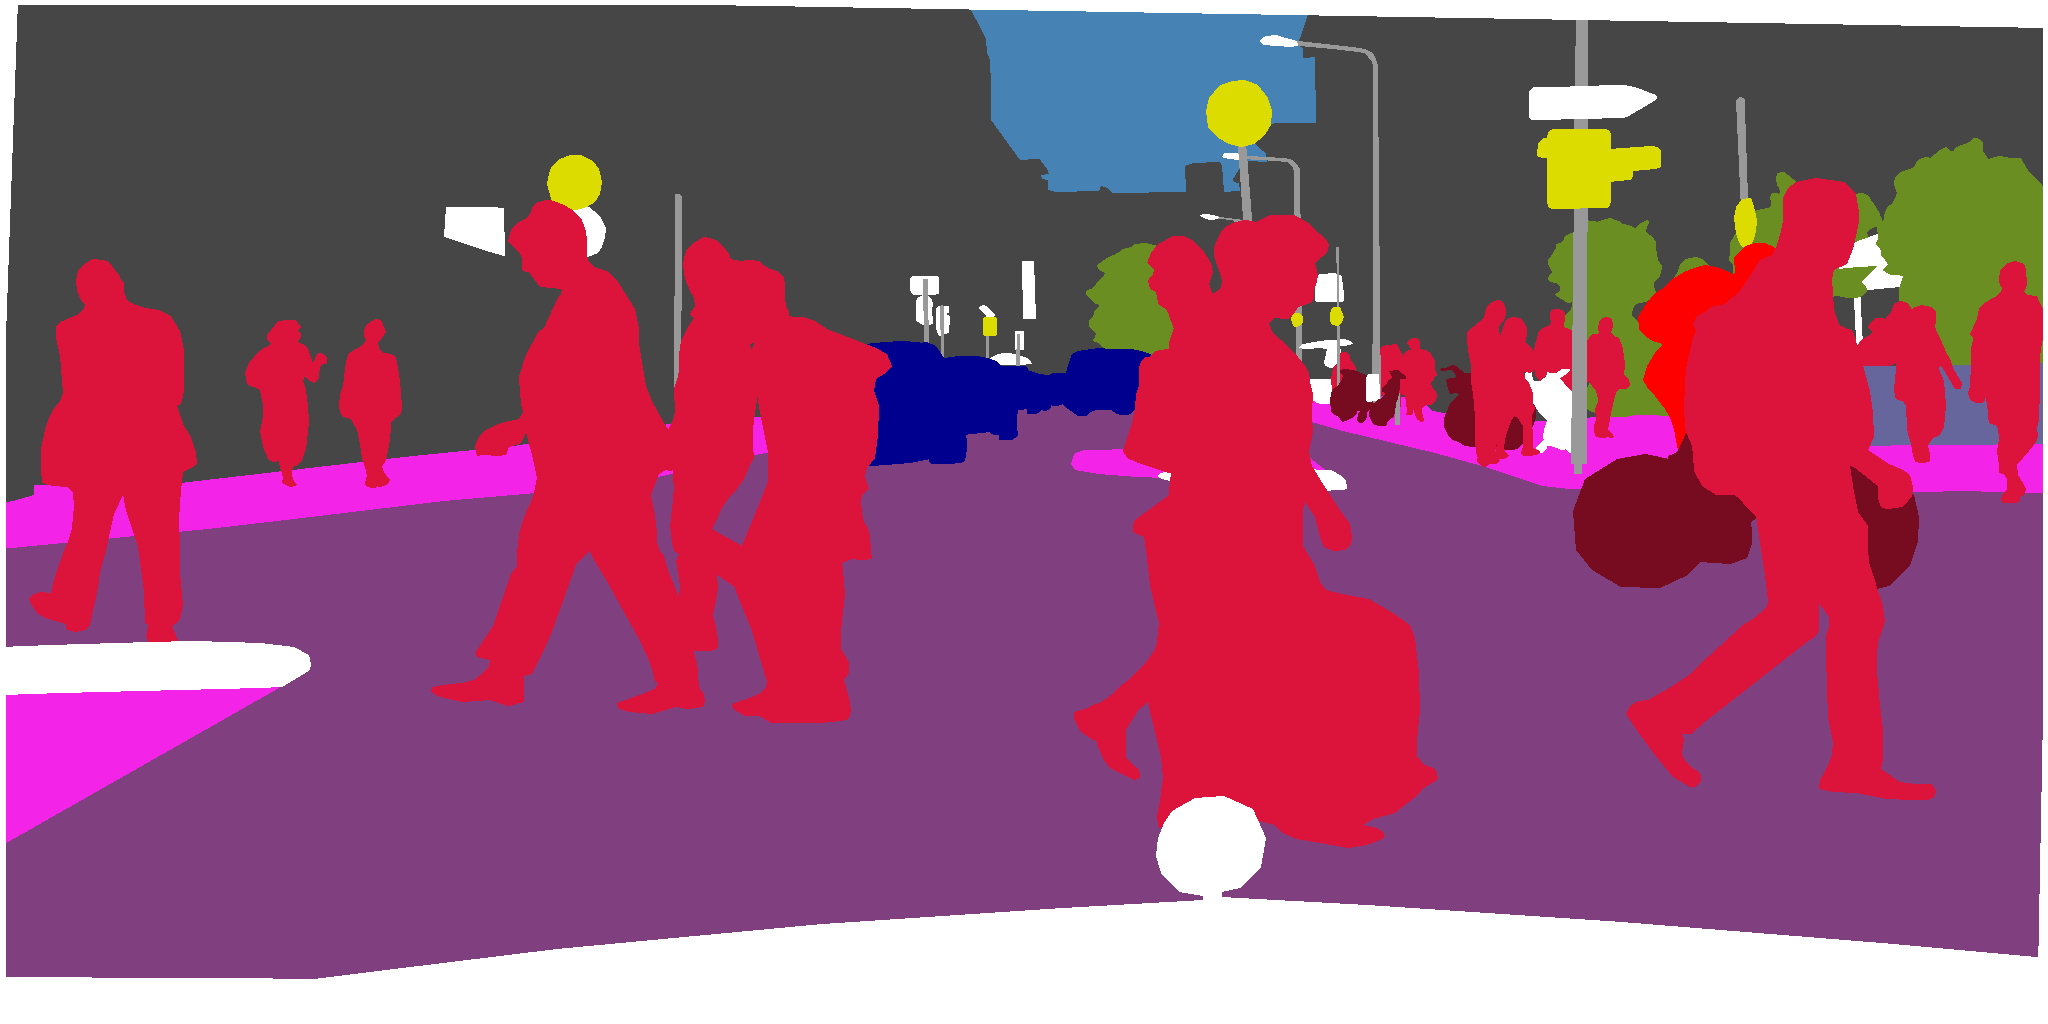
\includegraphics[width=\myw, height=\myh]{figs/gta2city_color/25_gt.png}
\\
   (a) Test Image & (b) Source Prediction & (c) CyCADA Prediction & (d) Ground Truth\\
  \end{tabular}
  }
  \caption{%\small 
  \textbf{GTA5 to CityScapes Semantic Segmentation.} Each test CityScapes image (a) along with the corresponding predictions from the source only model (b) and our CyCADA model (c) are shown and may be compared against the ground truth annotation (d). }
  \label{fig:gta-cityscapes-seg}
\end{figure}



\begin{table*}[h]
  \begin{center}
  \scriptsize
  \setlength{\tabcolsep}{1.35pt}
  \begin{tabular}{l|c|cccccccccccccccccccggg}
    \toprule
    \multicolumn{24}{c}{\textbf{GTA5 $\rightarrow$ Cityscapes}} \\
    \midrule
     &\rot{Architecture} & \rot{road} & \rot{sidewalk} & \rot{building} & \rot{wall} & \rot{fence} & \rot{pole} & \rot{traffic light} & \rot{traffic sign} & \rot{vegetation} & \rot{terrain} & \rot{sky} & \rot{person} & \rot{rider} & \rot{car} & \rot{truck} & \rot{bus} & \rot{train} & \rot{motorbike} & \rot{bicycle} & \rot{\textbf{mIoU}} & \rot{\textbf{fwIoU}} & \rot{\textbf{Pixel acc.}} \\ \midrule
    Source only & A            & 26.0 & 14.9 & 65.1 &  5.5 & 12.9 &  8.9 &  6.0 &  2.5 & 70.0 &  2.9 & 47.0 & 24.5 &  0.0 & 40.0 & 12.1 &  1.5 &  0.0 &  0.0 &  0.0 & 17.9 & 41.9 & 54.0 \\
    FCNs in the wild$^*$ & A & 70.4 & 32.4 & 62.1 & 14.9 &  5.4 & 10.9 & 14.2 &  2.7 & 79.2 & 21.3 & 64.6 & 44.1 &  4.2 & 70.4 &  8.0 &  7.3 &  0.0 &  3.5 &  0.0 & 27.1 & ---  & ---  \\
		%85.6	30.7	74.7	14.4	13.0	17.6	13.7	5.8	74.6	15.8	69.9	38.2	3.5	72.3	16.0	5.0	0.1	3.6	0.0
	CyCADA feat-only & A & \bf 85.6 &30.7& 74.7 &14.4 &13.0 &17.6 &13.7 &5.8 &74.6& 15.8 &\textbf{69.9} &38.2 &3.5 &72.3& 16.0& 5.0& 0.1 &3.6 &0.0& 29.2 & 71.5 & 82.5\\ %gta_fcn/adda/lr-1e-5_lambdaD-10_lambdaG-.1_rho-0.99_no_lsgan_weights_shared_discrim_feat_rot-0/net-iter5000.pth
	%
    CyCADA pixel-only & A & {83.5} & \textbf{38.3} & \textbf{76.4} & {20.6} & \textbf{16.5} &{22.2} & \textbf{26.2} & \textbf{21.9} & \textbf{80.4} & {28.7} & {65.7} & {49.4} &  4.2 & {74.6} & {16.0} & {26.6} &  {2.0} &  {8.0} &  0.0 & {34.8} & {73.1} & {82.8} \\
	%
	CyCADA pixel+feat & A & 85.2&	 37.2 	&\textbf{76.5} 	&\textbf{21.8} 	&15.0& 	\textbf{23.8}&	 22.9& 	21.5 	&\textbf{80.5} 	&\textbf{31.3} 	&60.7 	&\textbf{50.5} 	&\textbf{9.0}	 &\textbf{76.9} 	&\textbf{17.1} 	&\textbf{28.2} 	&\textbf{4.5} 	&\textbf{9.8} 	&0.0& \textbf{35.4} & \bf73.8 & \bf83.6\\ %cyclegta_fcn/adda/lr-1e-5_lambdaD-10_lambdaG-.1_rho-0.99_no_lsgan_weights_shared_discrim_feat_rot-0/net-2000
	\midrule
		Oracle - Target Super & A   & 96.4 & 74.5 & 87.1 & 35.3 & 37.8 & 36.4 & 46.9 & 60.1 & 89.0 & 54.3 & 89.8 & 65.6 & 35.9 & 89.4 & 38.6 & 64.1 & 38.6 & 40.5 & 65.1 & 60.3 & 87.6 & 93.1 \\
		\midrule
		\midrule
			Source only & B & 	42.7 &	26.3 &	51.7 &	5.5 &	6.8 &	13.8 &	23.6 &	6.9 &	75.5 &	11.5 &	36.8 &	49.3 &	0.9 &	46.7 &	3.4 &	5.0 &	0.0 &	5.0 &	1.4 & 21.7 &	47.4 &	62.5 \\
		CyCADA feat-only & B & 	78.1 &	31.1 &	71.2 &	10.3 &	14.1 &	29.8 &	28.1 &	20.9 &	74.0 &	16.8 &	51.9 &	53.6 &	6.1 &	65.4 &	8.2 &	20.9 &	1.8 &	13.9 &	5.9 & 31.7 &	67.4 &	78.4 \\
		 %results/gta5_to_cityscapes/adda_sgd/weights_unshared_nolsgan_discrim_score/drn26/lr1e-4_crop768_ld1_lg1/net-iter5000.pth
		 %
		CyCADA pixel-only & 	B & 63.7 &	24.7 &	69.3 &	21.2 &	17.0 &	30.3 &	33.0 &	
		\bf 32.0 &	80.5 &	25.3 &	62.3 &	62.0 &	\bf 15.1 &	73.1 &	19.8 &	23.6 &	5.5 &	16.2 &	\bf 28.7 & 37.0 &	63.8 &	75.4 \\ % drn26-cyclegta5-iter115000.pth 
		%
		CyCADA pixel+feat & B & \bf 79.1&	\bf 33.1&	\bf 77.9&	\bf 23.4&	\bf 17.3&	\bf 32.1&	\bf 33.3&	31.8& \bf	81.5&	\bf 26.7&	\bf 69.0	&\bf 62.8&	14.7&	\bf 74.5	&\bf 20.9	&\bf 25.6	&\bf 6.9&	\bf 18.8&	20.4 & \bf 39.5	&\bf 72.4&	\bf 82.3\\ %durian8:results/cyclegta5_to_cityscapes/adda_sgd/weights_shared_nolsgan_discrim_score/drn26/lr1e-5_crop768_ld1_lg0.1_momentum0.99/net-iter2975.pt
		\midrule
		Oracle - Target Super & B   & 97.3	&79.8&	88.6	&32.5&	48.2&	56.3&	63.6	&73.3	&89.0&	58.9&	93.0&	78.2&	55.2&	92.2&	45.0&	67.3&	39.6&	49.9&	73.6 & 67.4	& 89.6 & 94.3\\
    \bottomrule
  \end{tabular}
  \end{center}
  \caption{
    Adaptation between GTA5 and Cityscapes, showing IoU for each class and mean IoU, freq-weighted IoU and pixel accuracy.
    CyCADA significantly outperforms baselines, nearly closing the gap to the target-trained oracle on pixel accuracy. $^*$FCNs in the wild is by \citet{hoffman_arxiv16}. We compare our model using two base semantic segmentation architectures (A) VGG16-FCN8s~\citep{long_cvpr15} base network and (B) DRN-26~\citep{drn}.
    }
  \label{table:gta-cityscapes}
\end{table*}

\begin{table*}[h]
  \begin{center}
  \scriptsize
  \setlength{\tabcolsep}{1.35pt}
  \begin{tabular}{l|c|cccccccccccccccccccggg}
    \toprule
    \multicolumn{24}{c}{\textbf{GTA5 $\rightarrow$ Cityscapes}} \\
    \midrule
     &\rot{Architecture} & \rot{road} & \rot{sidewalk} & \rot{building} & \rot{wall} & \rot{fence} & \rot{pole} & \rot{traffic light} & \rot{traffic sign} & \rot{vegetation} & \rot{terrain} & \rot{sky} & \rot{person} & \rot{rider} & \rot{car} & \rot{truck} & \rot{bus} & \rot{train} & \rot{motorbike} & \rot{bicycle} & \rot{\textbf{mIoU}} & \rot{\textbf{fwIoU}} & \rot{\textbf{Pixel acc.}} \\ \midrule
    Source only & A            & 26.0 & 14.9 & 65.1 &  5.5 & 12.9 &  8.9 &  6.0 &  2.5 & 70.0 &  2.9 & 47.0 & 24.5 &  0.0 & 40.0 & 12.1 &  1.5 &  0.0 &  0.0 &  0.0 & 17.9 & 41.9 & 54.0 \\
    FCNs in the wild$^*$ & A & 70.4 & 32.4 & 62.1 & 14.9 &  5.4 & 10.9 & 14.2 &  2.7 & 79.2 & 21.3 & 64.6 & 44.1 &  4.2 & 70.4 &  8.0 &  7.3 &  0.0 &  3.5 &  0.0 & 27.1 & ---  & ---  \\
		%85.6	30.7	74.7	14.4	13.0	17.6	13.7	5.8	74.6	15.8	69.9	38.2	3.5	72.3	16.0	5.0	0.1	3.6	0.0
	CyCADA feat-only & A & \bf 85.6 &30.7& 74.7 &14.4 &13.0 &17.6 &13.7 &5.8 &74.6& 15.8 &\textbf{69.9} &38.2 &3.5 &72.3& 16.0& 5.0& 0.1 &3.6 &0.0& 29.2 & 71.5 & 82.5\\ %gta_fcn/adda/lr-1e-5_lambdaD-10_lambdaG-.1_rho-0.99_no_lsgan_weights_shared_discrim_feat_rot-0/net-iter5000.pth
	%
    CyCADA pixel-only & A & {83.5} & \textbf{38.3} & \textbf{76.4} & {20.6} & \textbf{16.5} &{22.2} & \textbf{26.2} & \textbf{21.9} & \textbf{80.4} & {28.7} & {65.7} & {49.4} &  4.2 & {74.6} & {16.0} & {26.6} &  {2.0} &  {8.0} &  0.0 & {34.8} & {73.1} & {82.8} \\
	%
	CyCADA pixel+feat & A & 85.2&	 37.2 	&\textbf{76.5} 	&\textbf{21.8} 	&15.0& 	\textbf{23.8}&	 22.9& 	21.5 	&\textbf{80.5} 	&\textbf{31.3} 	&60.7 	&\textbf{50.5} 	&\textbf{9.0}	 &\textbf{76.9} 	&\textbf{17.1} 	&\textbf{28.2} 	&\textbf{4.5} 	&\textbf{9.8} 	&0.0& \textbf{35.4} & \bf73.8 & \bf83.6\\ %cyclegta_fcn/adda/lr-1e-5_lambdaD-10_lambdaG-.1_rho-0.99_no_lsgan_weights_shared_discrim_feat_rot-0/net-2000
	\midrule
		Oracle - Target Super & A   & 96.4 & 74.5 & 87.1 & 35.3 & 37.8 & 36.4 & 46.9 & 60.1 & 89.0 & 54.3 & 89.8 & 65.6 & 35.9 & 89.4 & 38.6 & 64.1 & 38.6 & 40.5 & 65.1 & 60.3 & 87.6 & 93.1 \\
		\midrule
		\midrule
			Source only & B & 	42.7 &	26.3 &	51.7 &	5.5 &	6.8 &	13.8 &	23.6 &	6.9 &	75.5 &	11.5 &	36.8 &	49.3 &	0.9 &	46.7 &	3.4 &	5.0 &	0.0 &	5.0 &	1.4 & 21.7 &	47.4 &	62.5 \\
		CyCADA feat-only & B & 	78.1 &	31.1 &	71.2 &	10.3 &	14.1 &	29.8 &	28.1 &	20.9 &	74.0 &	16.8 &	51.9 &	53.6 &	6.1 &	65.4 &	8.2 &	20.9 &	1.8 &	13.9 &	5.9 & 31.7 &	67.4 &	78.4 \\
		 %results/gta5_to_cityscapes/adda_sgd/weights_unshared_nolsgan_discrim_score/drn26/lr1e-4_crop768_ld1_lg1/net-iter5000.pth
		 %
		CyCADA pixel-only & 	B & 63.7 &	24.7 &	69.3 &	21.2 &	17.0 &	30.3 &	33.0 &	
		\bf 32.0 &	80.5 &	25.3 &	62.3 &	62.0 &	\bf 15.1 &	73.1 &	19.8 &	23.6 &	5.5 &	16.2 &	\bf 28.7 & 37.0 &	63.8 &	75.4 \\ % drn26-cyclegta5-iter115000.pth 
		%
		CyCADA pixel+feat & B & \bf 79.1&	\bf 33.1&	\bf 77.9&	\bf 23.4&	\bf 17.3&	\bf 32.1&	\bf 33.3&	31.8& \bf	81.5&	\bf 26.7&	\bf 69.0	&\bf 62.8&	14.7&	\bf 74.5	&\bf 20.9	&\bf 25.6	&\bf 6.9&	\bf 18.8&	20.4 & \bf 39.5	&\bf 72.4&	\bf 82.3\\ %durian8:results/cyclegta5_to_cityscapes/adda_sgd/weights_shared_nolsgan_discrim_score/drn26/lr1e-5_crop768_ld1_lg0.1_momentum0.99/net-iter2975.pt
		\midrule
		Oracle - Target Super & B   & 97.3	&79.8&	88.6	&32.5&	48.2&	56.3&	63.6	&73.3	&89.0&	58.9&	93.0&	78.2&	55.2&	92.2&	45.0&	67.3&	39.6&	49.9&	73.6 & 67.4	& 89.6 & 94.3\\
    \bottomrule
  \end{tabular}
  \end{center}
  \caption{
    Adaptation between GTA5 and Cityscapes, showing IoU for each class and mean IoU, freq-weighted IoU and pixel accuracy.
    CyCADA significantly outperforms baselines, nearly closing the gap to the target-trained oracle on pixel accuracy. $^*$FCNs in the wild is by \citet{hoffman_arxiv16}. We compare our model using two base semantic segmentation architectures (A) VGG16-FCN8s~\citep{long_cvpr15} base network and (B) DRN-26~\citep{drn}.
    }
  \label{table:gta-cityscapes}
\end{table*}

\subsubsection{Synthetic to real adaptation}

To evaluate our method's applicability to real-world adaptation settings, we investigate adaptation from synthetic to real-world imagery.
The results of this evaluation are presented in Table~\ref{table:gta-cityscapes} with qualitative results shown in Figure~\ref{fig:gta-cityscapes-seg}.
Once again, CyCADA achieves state-of-the-art results, recovering approximately 40\% of the performance lost to domain shift.
CyCADA also improves or maintains performance on all 19 classes.
Examination of fwIoU and pixel accuracy as well as individual class IoUs reveals that our method performs well on most of the common classes.
Although some classes such as \emph{train} and \emph{bicycle} see little or no improvement, we note that those classes are poorly represented in the GTA5 data, making recognition very difficult. We compare our model against \citet{shrivastava_cvpr17} for this setting, but found this approach did not converge and resulted in worse performance than the source only model (see Appendix for full details).

We visualize the results of image-space adaptation between GTA5 and Cityscapes in Figure~\ref{fig:gta-cityscapes}.
The most obvious difference between the original images and the adapted images is the saturation levels---the GTA5 imagery is much more vivid than the Cityscapes imagery, so adaptation adjusts the colors to compensate.
We also observe texture changes, which are perhaps most apparent in the road: in-game, the roads appear rough with many blemishes, but Cityscapes roads tend to be fairly uniform in appearance, so in converting from GTA5 to Cityscapes, our model removes most of the texture.
Somewhat amusingly, our model has a tendency to add a hood ornament to the bottom of the image, which, while likely irrelevant to the segmentation task, serves as a further indication that image-space adaptation is producing reasonable results.
